\section{Results}

\subsection{Comparison}

\begin{frame}{Objectives}{Comparison}
\begin{columns}
	\column{0.35\textwidth}
	{\Large Minimize distance}
	\begin{figure}
		\centering
		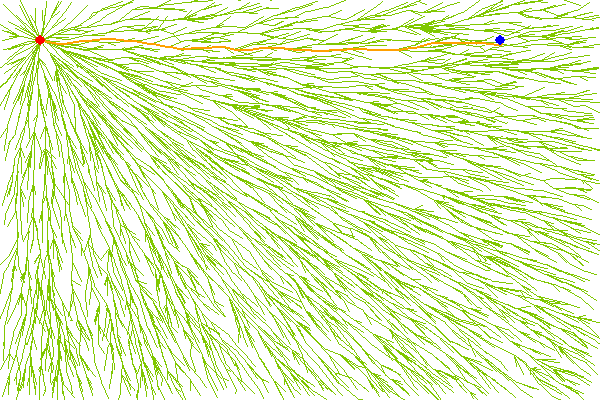
\includegraphics[width=\linewidth]{figure/sim2-2obj/MORRTstar00-0.png}
		%\caption{}
		\label{fig:sim:01:prob1}
	\end{figure}
	\column{0.35\textwidth}
	{\Large Minimize cost}
	\begin{figure}
		\centering
		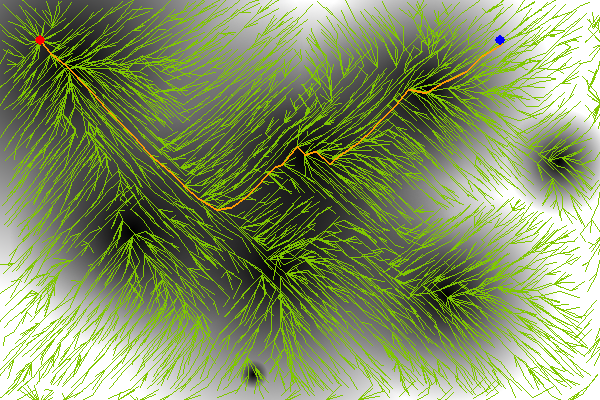
\includegraphics[width=\linewidth]{figure/sim2-2obj/MORRTstar00-1.png}
		%\caption{}
		\label{fig:sim:01:prob2}
	\end{figure}
\end{columns}
\end{frame}

\begin{frame}{Solutions}{Comparison}
\begin{columns}
	\column{0.33\textwidth}
	{ Weight-sum approach}
	\begin{figure}
		\centering
		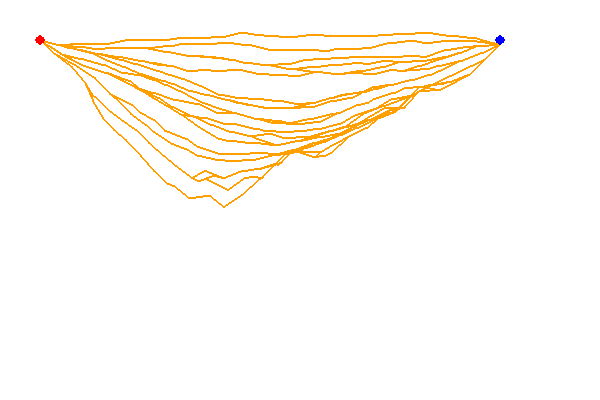
\includegraphics[width=\linewidth]{figure/sim1-2obj/MORRTstar00-ALL.png}
		%\caption{}
		\label{fig:sim:01:sol1}
	\end{figure}
	\column{0.33\textwidth}
	{ NSGA-II \newline}
	\begin{figure}
		\centering
		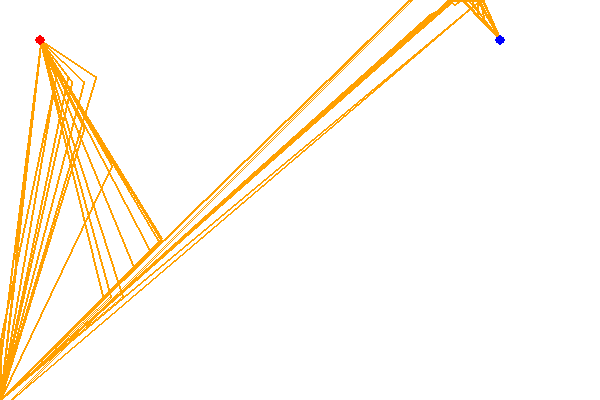
\includegraphics[width=\linewidth]{figure/sim3-2obj/MOPath01-ALL.png}
		%\caption{}
		\label{fig:sim:01:sol2}
	\end{figure}
	\column{0.33\textwidth}
	{ Tchebycheff approach}
	\begin{figure}
		\centering
		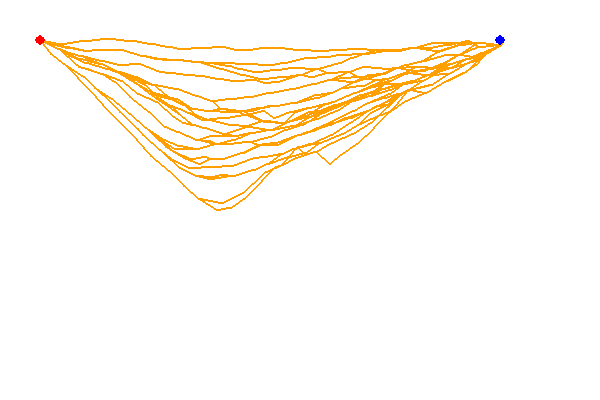
\includegraphics[width=\linewidth]{figure/sim2-2obj/MORRTstar00-ALL.png}
		%\caption{}
		\label{fig:sim:01:sol3}
	\end{figure}
\end{columns}
\end{frame}

\begin{frame}{Fitness}{Comparison}
\begin{columns}
	\column{0.33\textwidth}
	{ Weight-sum approach}
	\begin{figure}
		\centering
		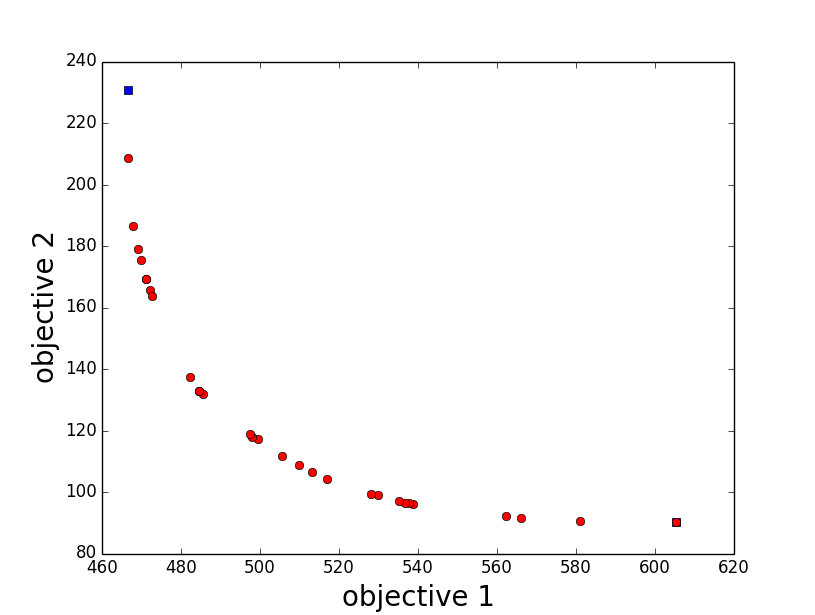
\includegraphics[width=\linewidth]{figure/sim1-2obj/PF01-MORRT.png}
		%\caption{}
		\label{fig:sim:01:fit1}
	\end{figure}
	\column{0.33\textwidth}
	{ NSGA-II \newline}
	\begin{figure}
		\centering
		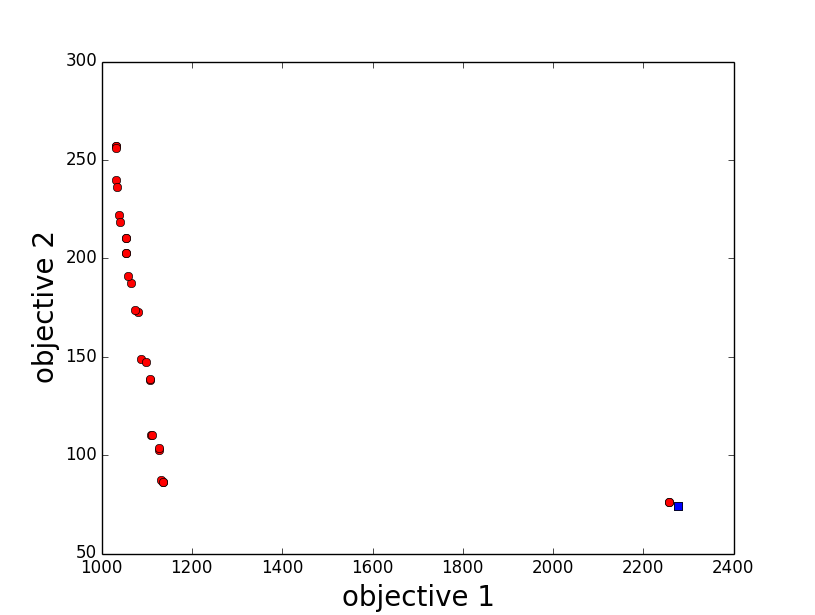
\includegraphics[width=\linewidth]{figure/sim3-2obj/PF03-MOPATH.png}
		%\caption{}
		\label{fig:sim:01:fit2}
	\end{figure}
	\column{0.33\textwidth}
	{ Tchebycheff approach}
	\begin{figure}
		\centering
		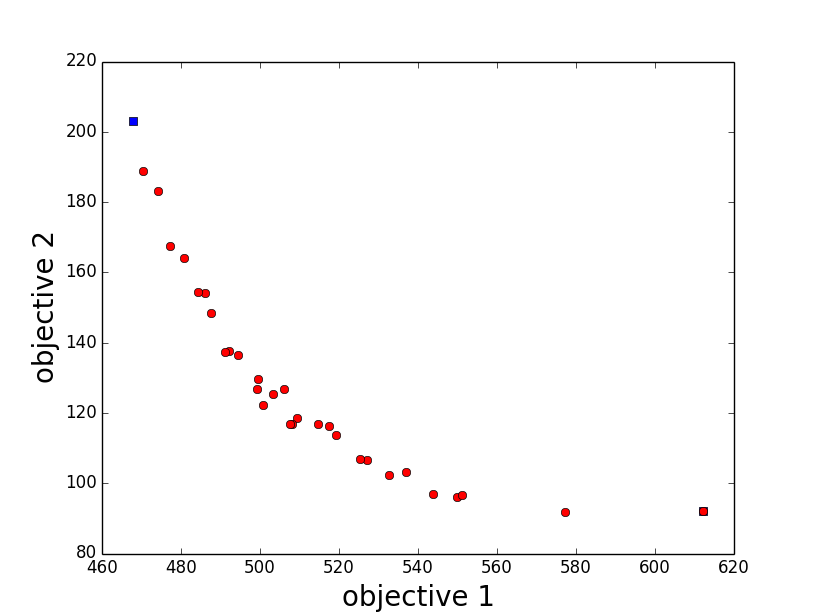
\includegraphics[width=\linewidth]{figure/sim2-2obj/PF02-MORRT2.png}
		%\caption{}
		\label{fig:sim:01:fit3}
	\end{figure}
\end{columns}
\end{frame}

\subsection{Obstacles}

\begin{frame}{Objectives}{Obstacles}
\begin{columns}
	\column{0.4\textwidth}
	{ Minimize distance}
	\begin{figure}
		\centering
		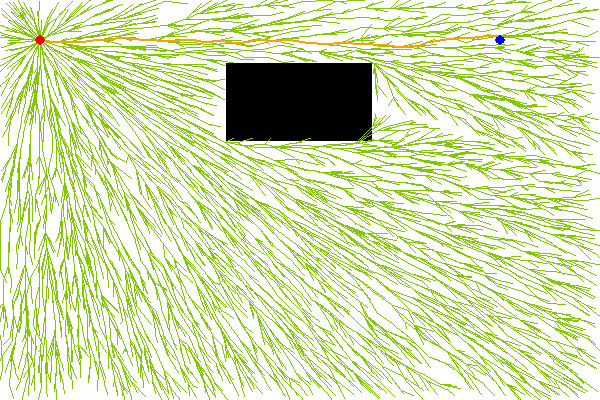
\includegraphics[width=\linewidth]{figure/sim5-obstacle/MORRTstar01-1-0.png}
		%\caption{}
		\label{fig:sim:02:prob1}
	\end{figure}
	\column{0.4\textwidth}
	{ Minimize cost}
	\begin{figure}
		\centering
		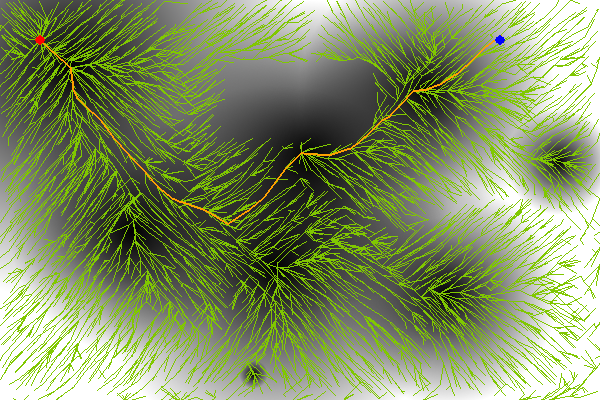
\includegraphics[width=\linewidth]{figure/sim5-obstacle/MORRTstar01-1-1.png}
		%\caption{}
		\label{fig:sim:02:prob2}
	\end{figure}
\end{columns}
\end{frame}

\begin{frame}{Solutions}{Obstacles}
\begin{columns}
	\column{0.4\textwidth}
	{ Weight-sum approach}
	\begin{figure}
		\centering
		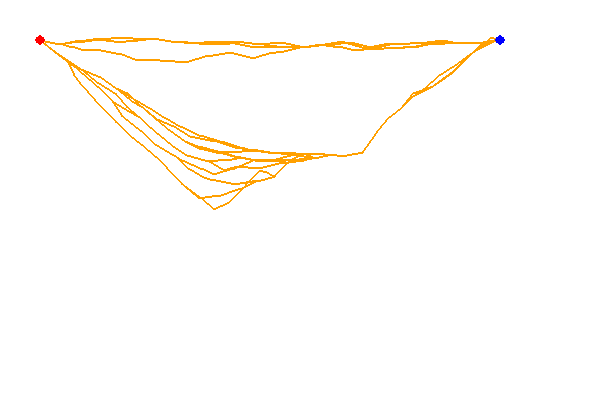
\includegraphics[width=\linewidth]{figure/sim4-obstacle/MORRTstar01-1-ALL.png}
		%\caption{}
		\label{fig:sim:02:sol1}
	\end{figure}
	\column{0.4\textwidth}
	{ Tchebycheff approach}
	\begin{figure}
		\centering
		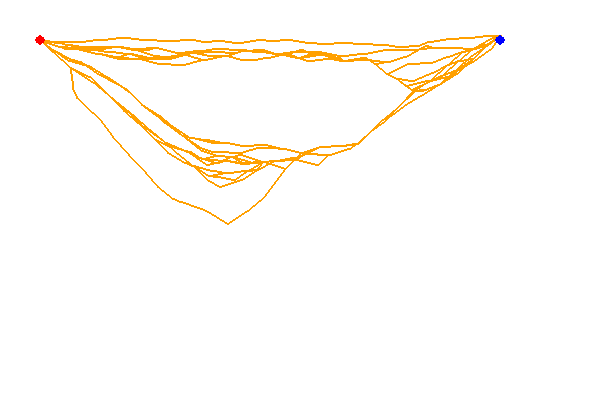
\includegraphics[width=\linewidth]{figure/sim5-obstacle/MORRTstar01-1-ALL.png}
		%\caption{}
		\label{fig:sim:02:sol2}
	\end{figure}
\end{columns}
\end{frame}

\begin{frame}{Fitness}{Obstacles}
\begin{columns}
	\column{0.4\textwidth}
	{ Weight-sum approach}
	\begin{figure}
		\centering
		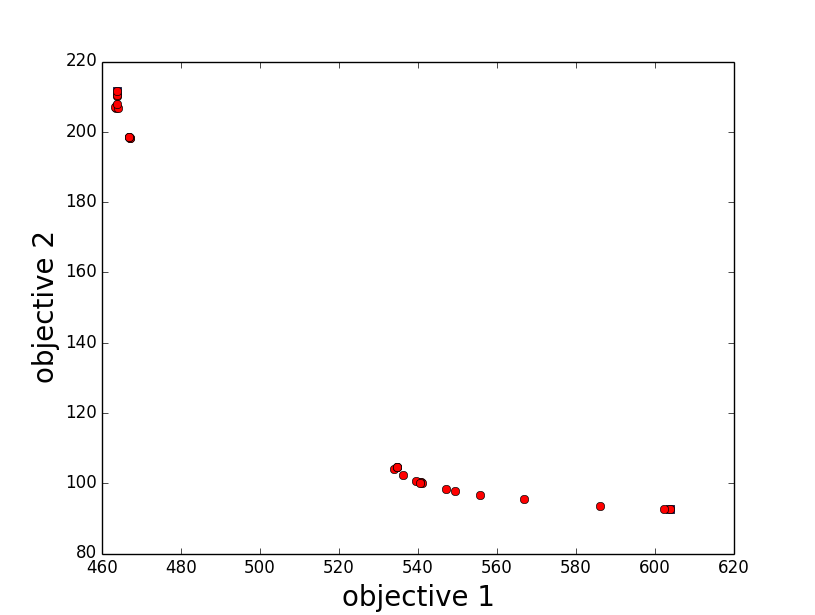
\includegraphics[width=\linewidth]{figure/sim4-obstacle/PF04-MORRT.png}
		%\caption{}
		\label{fig:sim:02:fit1}
	\end{figure}
	\column{0.4\textwidth}
	{ Tchebycheff approach}
	\begin{figure}
		\centering
		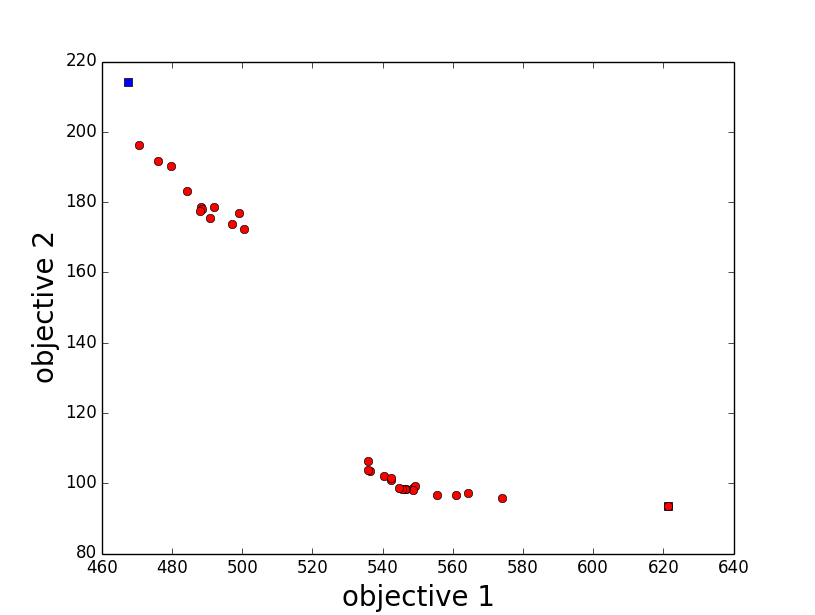
\includegraphics[width=\linewidth]{figure/sim5-obstacle/PF05-MORRT2.png}
		%\caption{}
		\label{fig:sim:02:fit2}
	\end{figure}
\end{columns}
\end{frame}

\subsection{More objectives}

\begin{frame}{Objectives}{More objectives}
\begin{columns}
	\column{0.33\textwidth}
	{ Minimize distance}
	\begin{figure}
		\centering
		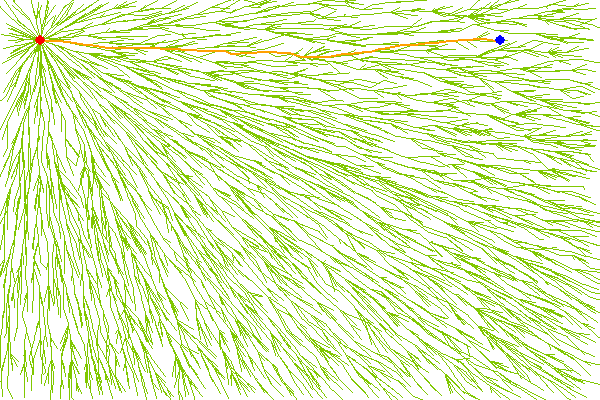
\includegraphics[width=\linewidth]{figure/sim7-3obj/MORRTstar02-0.png}
		%\caption{}
		\label{fig:sim:03:prob1}
	\end{figure}
	\column{0.33\textwidth}
	{ Minimize cost 1}
	\begin{figure}
		\centering
		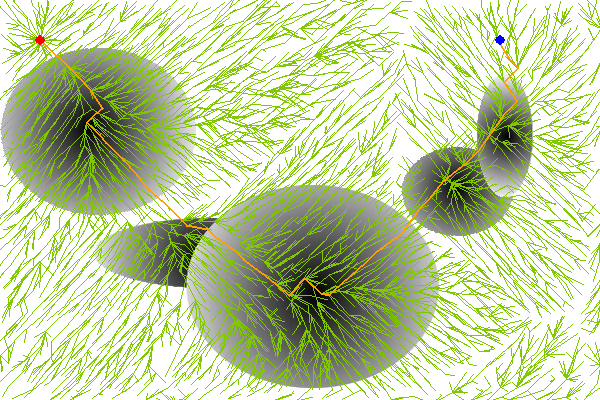
\includegraphics[width=\linewidth]{figure/sim7-3obj/MORRTstar02-1.png}
		%\caption{}
		\label{fig:sim:03:prob2}
	\end{figure}
	\column{0.33\textwidth}
	{ Minimize cost 2}
	\begin{figure}
		\centering
		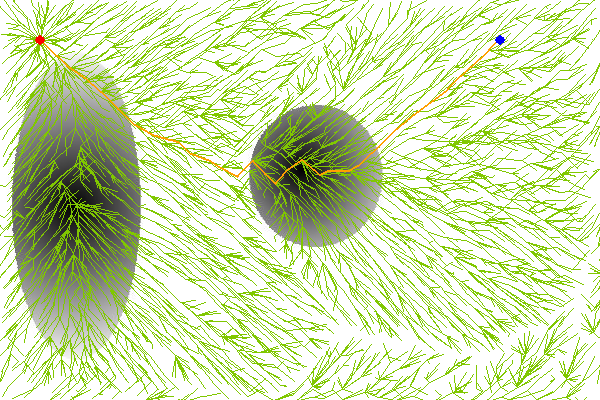
\includegraphics[width=\linewidth]{figure/sim7-3obj/MORRTstar02-2.png}
		%\caption{}
		\label{fig:sim:03:prob3}
	\end{figure}
\end{columns}
\end{frame}

\begin{frame}{Solutions}{More objectives}
\begin{columns}
	\column{0.4\textwidth}
	{ Weight-sum approach}
	\begin{figure}
		\centering
		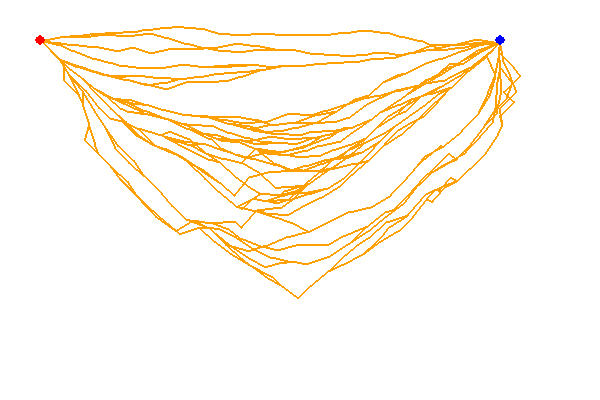
\includegraphics[width=\linewidth]{figure/sim6-3obj/MORRTstar02-ALL.png}
		%\caption{}
		\label{fig:sim:03:sol1}
	\end{figure}
	\column{0.4\textwidth}
	{ Tchebycheff approach}
	\begin{figure}
		\centering
		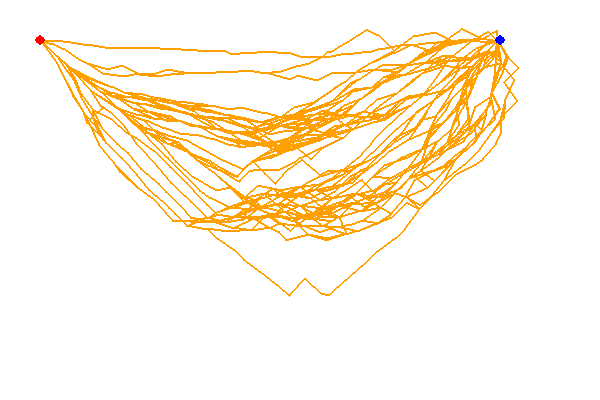
\includegraphics[width=\linewidth]{figure/sim7-3obj/MORRTstar02-ALL.png}
		%\caption{}
		\label{fig:sim:03:sol2}
	\end{figure}
\end{columns}
\end{frame}

\begin{frame}{Fitness}{More objectives}
\begin{columns}
	\column{0.4\textwidth}
	{ Weight-sum approach}
	\begin{figure}
		\centering
		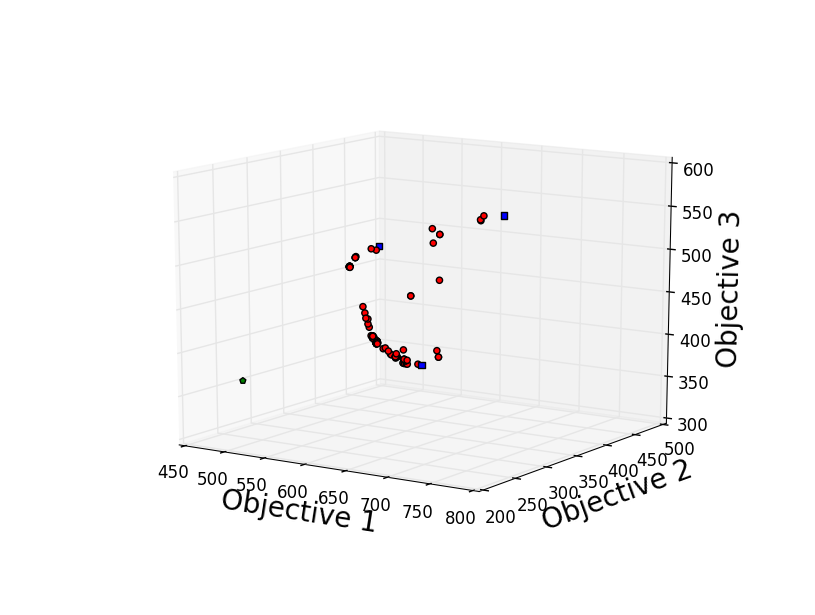
\includegraphics[width=\linewidth]{figure/sim6-3obj/PF06-MORRT.png}
		%\caption{}
		\label{fig:sim:03:fit1}
	\end{figure}
	\column{0.4\textwidth}
	{ Tchebycheff approach}
	\begin{figure}
		\centering
		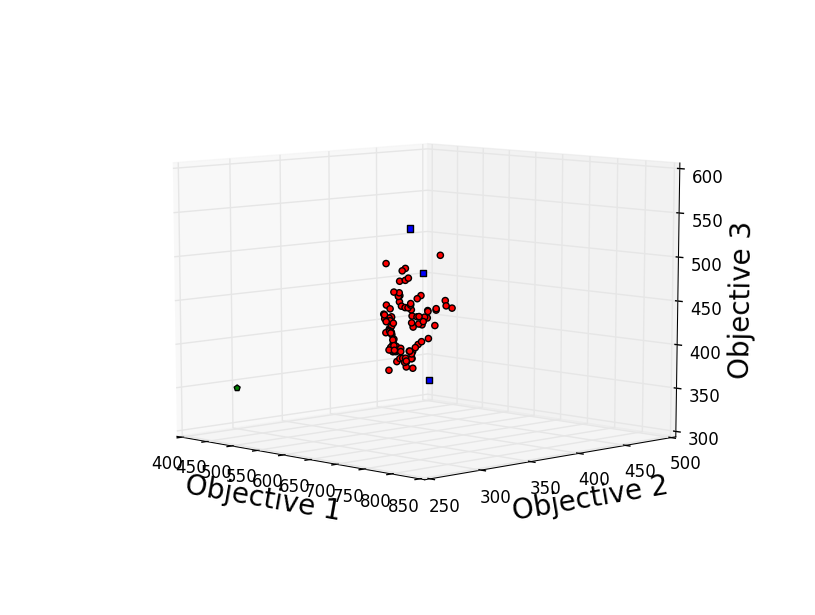
\includegraphics[width=\linewidth]{figure/sim7-3obj/PF07-MORRT2.png}
		%\caption{}
		\label{fig:sim:03:fit2}
	\end{figure}
\end{columns}
\end{frame}